\section{Forces}
\subsection{Types of force}
\begin{defn}{Hooke's Law}{}
Force is directly proportional to extension of a spring, provided that the \underline{elastic limit} has not been exceeded; that is, $\vb{F}\propto\vb{x}$.
\begin{equation}
\vb{F}=k\vb{x}
\end{equation}
where $k$ is the \textbf{spring constant}.
\end{defn}

\begin{itemize}
\item For springs in \textbf{parallel}, 
\begin{equation} k_{\text{eff}} = \sum_{i} k_i \end{equation}
\item For springs in \textbf{series},
\begin{equation} \frac{1}{k_{\text{eff}}} = \sum_{i} \frac{1}{k_i} \end{equation}
\end{itemize}

\textbf{Elastic potential energy} is stored in an object when it undergoes deformation (e.g. when a spring is extended or compressed).
\begin{equation} U = \frac{1}{2}Fx = \frac{1}{2}kx^2 \end{equation}
Graphically, elastic potential energy is the area under a force-extension graph.
\[ W = \int F \dd{x} \]

\subsection{Upthrust}
\textbf{Pressure} $P$ of a liquid column is given by 
\begin{equation}
P=\rho gh
\end{equation}

\deriv{See Appendix for the derivation.}

\begin{defn}{Upthrust $\vb{U}$}{}
Vertical upward force exerted by the surrounding fluid when a body is submerged, fully or partially, in a fluid.
\end{defn} 

\begin{remark}
Origin of upthrust: Upthrust is the \underline{resultant} force due to the difference in pressure exerted by fluid at the top and bottom surfaces of the body.
\end{remark}

\begin{defn}{Archimedes' Principle}{}
Upthrust is \underline{equal in magnitude}, \underline{opposite in direction} to the weight of fluid displaced by the body.
\begin{equation}
\vb{U}=\vb{W}_{\text{displaced}}=\rho_{\text{fluid}}\, V_{\text{displaced}}\,g
\end{equation}
\end{defn}

\deriv{See Appendix for the derivation.}

For an object floating in equilibrium, upthrust is equal in magnitude, opposite in direction to weight of the object.
\begin{equation}
\vb{U}=\vb{W}_{\text{object}}
\end{equation}

\subsection{Centre of gravity}
\begin{defn}{Centre of gravity}{}
A single point where the entire weight of the object may be taken as acting at.
\end{defn} 

\subsection{Turning effects of forces}
\begin{defn}{Moment of a force}{}
Product of magnitude of the force and perpendicular distance of the \emph{line of action} of the force from the pivot point.
\begin{equation} M = F \times \perp d \end{equation}
\end{defn}

\begin{defn}{Couple}{}
A pair of forces of \underline{equal magnitude} but acting in \underline{opposite directions} whose lines of action are \underline{parallel but separate}.
\end{defn} 

\begin{remark}
A couple is a pair of forces which tends to produce \emph{rotation} only.
\end{remark}

\begin{defn}{Torque of a couple}{}
Product of one of the forces and the perpendicular distance between the forces.
\begin{equation} \tau = F \times \perp d \end{equation}
\end{defn}

\begin{defn}{Principle of Moments}{}
When a system is in equilibrium, sum of clockwise moments \underline{about any axis} must be equal to sum of anticlockwise moments \underline{about the same axis}.
\begin{equation} \sum \text{ clockwise moments} = \sum \text{ anticlockwise moments} \end{equation}
\end{defn} 
\pagebreak

\subsection{Equilibrium of forces}
A system is in equilibrium when there is 
\begin{itemize}
\item no resultant force, and
\item no resultant torque
\end{itemize}

\begin{defn}{Translational equilibrium}{}
Net force is zero \underline{in any direction}.
\[ \sum\vb{F}=\vb{0} \]
\end{defn} 

\begin{defn}{Rotational equilibrium}{}
Net torque is zero \underline{about any axis of rotation}. 
\[ \sum\mathbf{\tau}=\vb{0} \]
\end{defn}

For multiple non-parallel forces, this is illustrated by: 
\begin{itemize}
\item Forces form a \textbf{closed vector polygon}.
\item Lines of actions of forces \textbf{intersect at one point}, so that there is no resultant moment about their point of intersection.
\end{itemize}
\pagebreak

\subsection{Problems}
\begin{prbm}
Explain why the upthrust acting on a human body when in air is normally ignored.
\end{prbm}
\begin{proof}[Answer]
The average person weighs about $600\:\unit{N}$. Upthrust by air is about $1\:\unit{N}$, less than $0.2\%$ of the weight of the person.
\end{proof}

\begin{prbm}
Why can a lump of plasticine moulded into the shape of a bowl float in water?
\end{prbm}
\begin{proof}[Answer]
Bowl is able to displace a greater volume of water.

If the plasticine floats, 
\[ W = U \]
\[ \rho_{\mathrm{plasticine}} g V_{\mathrm{plasticine}} = p_{\mathrm{water}} g V_{\mathrm{water\:displaced}} \]

Since $p_{\mathrm{plasticine}} > \rho_{\mathrm{water}}$, in order for the plasticine to float, $V_{\mathrm{water\:displaced}} > V_{\mathrm{plasticine}}$.

Hence plasticine must be able to displace a larger volume of water than its own volume.
\end{proof}
\pagebreak

\begin{prbm}
A rope is connected to a vertical wall at one end, and a horizontal external force $F=15.0\:\unit{N}$ pulls on the other end. The rope is in equilibrium and makes an angle $\theta = 25.0\degree$ with the wall. What is the weight $W$ of the rope? 

\textit{Leave your answer to $3$ significant figures in units of \emph{N}}.

\begin{figure}[H]
    \centering
    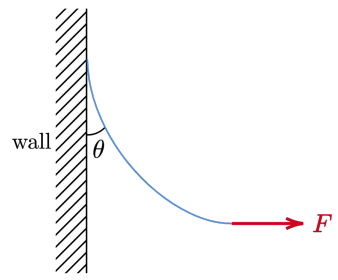
\includegraphics{images/Mysterious_Rope.png}
\end{figure}
\end{prbm}

\begin{proof}[Solution]
Since the rope makes an angle $\theta$ with the wall, and the tension in the rope acts along the rope, we can write the following force balance equations for the horizontal and vertical axes respectively:
\[ T \sin \theta = F \]
\[ T \cos \theta = W \]
Hence solving for $W$,
\begin{align*}
W &= \frac{F \cos \theta}{\sin \theta} \\
W &= F \cot \theta \\
\Aboxed{W &\approx 32.2\:\unit{N}}
\end{align*}
\end{proof}
\pagebreak

\begin{prbm}[Sailor capstan]
A capstan is a device used aboard ships in order to control a rope that is under great tension. The rope is wrapped around a fixed drum of radius $R$, usually for several turns. The load on the rope pulls it with a force $T_A$, and the sailor holds the other end of the rope with a much smaller force $T_B$. The coefficient of static friction between the rope and the drum is $\mu_s$. The sailor is holding the rope so that it is just about to slip.

\begin{figure}[H]
    \centering
    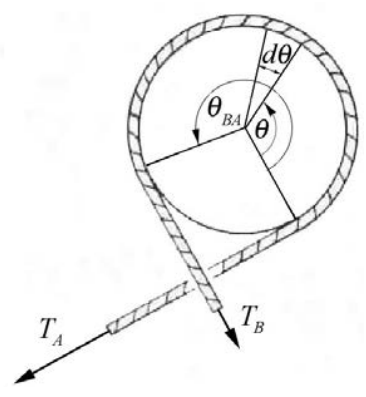
\includegraphics[width=6cm]{images/Capstan.png}
\end{figure}

Show that \[ T_B = T_Ae^{-\mu_s \theta_{BA}}\]
where $\theta_{BA}$ is the angle subtended by the rope on the drum. 
\end{prbm}

\begin{proof}[Solution]
Analysing forces on a small slice of rope of arc length $R\Delta\theta$:

\begin{figure}[H]
    \centering
    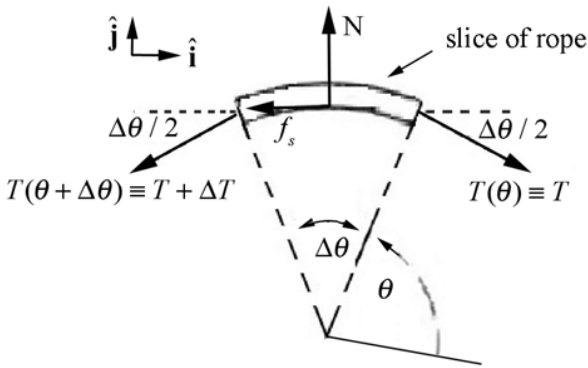
\includegraphics[width=8cm]{images/Capstan_1.png}
\end{figure}

In the horizontal direction,
\[ T\cos\frac{\Delta\theta}{2} - \brac{T+\Delta T}\cos\frac{\Delta\theta}{2} - f_s = 0 \]
In the vertical direction,
\[ N - T\sin\frac{\Delta\theta}{2} - \brac{T+\Delta T}\sin\frac{\Delta\theta}{2} = 0 \]

Solving the two equations simultaneously gives us 
\[ \frac{\Delta T}{\Delta \theta} = \mu_s T \]
As $\Delta \theta \to 0$, 
\[ \dv{T}{\theta} = -\mu_s T \]
Solving the differential equation,
\begin{align*}
\int_{T_A}^{T_B} \frac{1}{T} \dd{T} 
&= -\mu_s \int_{\theta_A}^{\theta_B} \dd{\theta} \\
\ln \frac{T_B}{T_A} &= -\mu_s\brac{\theta_B-\theta_A} \\
\Aboxed{T_B &= T_A e^{-\mu_s \theta_{BA}}}
\end{align*}

The exponential dependence suggests that the coefficient $e^{-\mu_s\theta_{BA}}$ becomes very small when $\theta_{BA}$ increases. Note that for $n$ turns of the rope, $\theta_{BA}=2\pi n\:\unit{rad}$.
\end{proof}
\pagebreak

\begin{prbm}[Yoyo problem]

\end{prbm}

\begin{proof}[Solution]

\end{proof}
\pagebreak

\begin{prbm}
What is the minimum force $F$ that must be applied to cause the cylinder to barely lift up off of the bottom step and rotate up around the corner of the next one? Assume that the cylinder does not slip on the corner of the next step.
\end{prbm}

\begin{figure}[H]
    \centering
    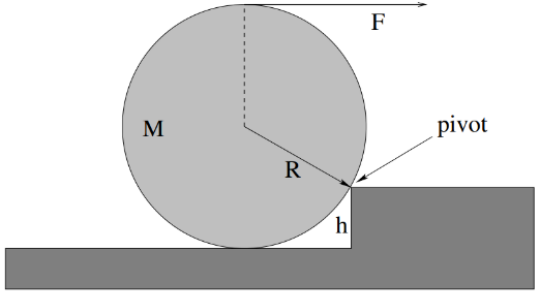
\includegraphics[width=10cm]{images/Cylinder_moment.png}
\end{figure}

\begin{proof}[Solution]
Computing the torques of $F$ and $Mg$ gives us 
\[ \boxed{F=\frac{Mg\sqrt{R^2-(R-h)^2}}{2R-h}} \]
\end{proof}

\pagebreak